\chapter{Test Bench}
One of the development steps is the verification of the design. It is very important to determine whether the requirements of the systems specification are met. There are generally two approaches to validate systems functionality. The formal verification is a mathematical prove of the compatibility between the specification and systems function. The verification through simulation focuses on testing the design and  ...

\section{General Overview}
The main idea behind the test bench development was to make it configurable and adaptable. The test bench has been developed parallel to the system and therefore has been redesigned to suit the current needs. It became clear that it has to be a test bench able to conduct various test on designs with various input ranges with various frequencies and not be bound to one design or interface. The general ideas of testing a design is shown in \autoref{fig:test}.

\begin{figure}[H]
\centering
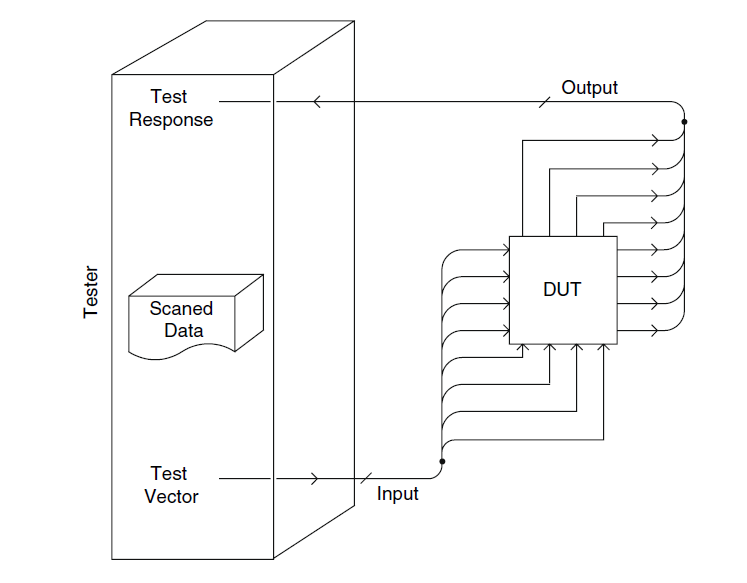
\includegraphics[width=0.65\textwidth]{figures/test.png}
\caption{The tester principle~\cite{book:Navabi}}
\label{fig:test}
\end{figure}

The tester is responsible for test vector generation, feeding the vectors to the inputs of the Device Under Test (DUT), gathering the response and evaluating it. Both generation and evaluation tasks are very design dependent and have to be adjusted after the design is placed in the test bench. The easiest interface from the users perspective is a PC application acting as the GUI. Since the UUT is being developed on the RTL level with hardware description language and the test bench is supposed to test it for real working frequencies, at least as close as possible to real environment, implementation on an FPGA would allow such test. The feeding and gathering has to also be implemented in FPGA as physical test interface. The middleware, responsible for the communication and translation of signals, should support standard communication protocols for data exchange with PC and hardware interface to the FPGA. The rough design draft is shown in the figure \autoref{fig:draft}.\\
 

\begin{figure}[H]
\centering
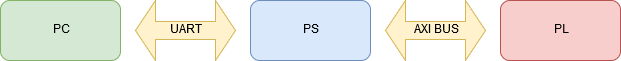
\includegraphics[width=0.65\textwidth]{figures/PCPSPL.png}
\caption{Draft of the test system}
\label{fig:draft}
\end{figure}

\section {Target Architecture}
The target architecture chosen is the Xilinx Zynq SoC (system on Chip). The idea of integrating processors, memories, mixed signal components with RF components in one chip has been known for a long time. Such Application Specific Integrated Circuits (ASICs) are designed to reduce size, to target more secure and faster communication between systems, to lower power consumption and increase reliability. The production cost of a single ASIC is also lower. The main problem of such full custom design is lack of flexibility, high, non-recurring development cost and time. Another important drawback is the lack of compatibility with most of standard applications which speed up the development process and, what comes with it, the time to market. Instead of full-custom ASICs, the semi custom SoCs with programmable logic are gaining on importance. Standard processors connected with Field Programmable Arrays (FPGAs), peripherlas and communication systems create an All-Pogrammable-System-on-Chip. The Programmable Logic is ideal for implementing high-speed logic and data flow systems, while Processing System supports operating system and standard software routines.The combination allows the developer to apply any system and easily partition it between hardware and software.

The Xilinx Zynq XC7Z020-1-CLG484 produced in 28nm technology is a SoC solution containing an ARM hardware processor with two cores and an FPGA with 53200 LUTs, 106400 DFFs and 560 KB of Block RAM. It supports all common standard communication interfaces: UART, SPI, CAN, I2C, GigE, GPIO and SDIO . It also allows quick data transfers between Pocessing System (PS) and Programmable Logic (PL) thanks to Xilinx AXI Bus. The full overview of the Zynq architecture is shown in \autoref{fig:Zynq}. The platform suits all needs of the hardware and middleware layer of the test bench.

\begin{figure}[H]
\centering
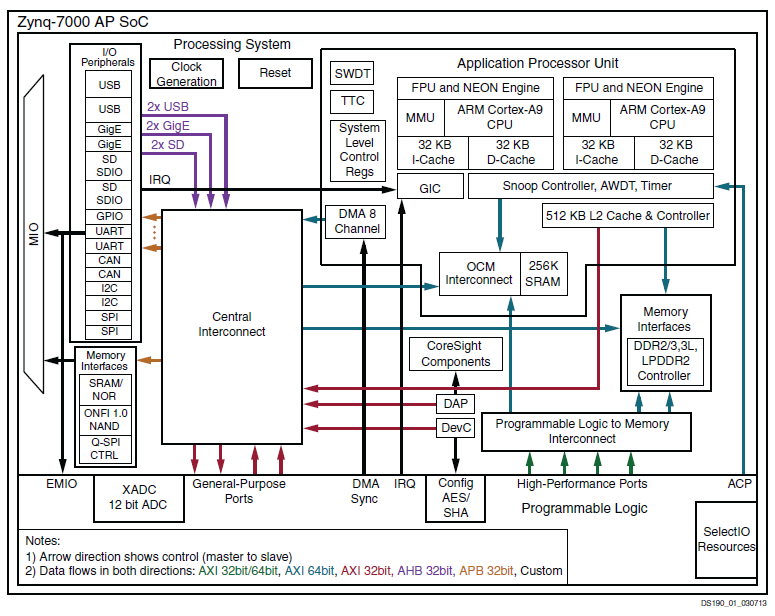
\includegraphics[width=0.65\textwidth]{figures/Zynq.png}
\caption{The Zynq Processing System~\cite{book:ZynqBook}}
\label{fig:Zynq}
\end{figure}

\section{Physical Interface}
\section{Middleware}
\section{GUI}